% ============================================================
% Teacher Architecture: Full Mathematical Derivation
% Shrink or Sink 2025 — ResNet-50 Ultimate Teacher
% ============================================================
\documentclass[12pt, a4paper]{article}

% ── Packages ──────────────────────────────────────────────────
\usepackage[T1]{fontenc}
\usepackage{lmodern}
\usepackage{amsmath, amssymb, mathtools}
\usepackage{geometry}
\usepackage{graphicx}
\usepackage{booktabs}
\usepackage{hyperref}
\usepackage{xcolor}
\usepackage{algorithm}
\usepackage{algpseudocode}
\usepackage{tikz}
\usepackage{pgfplots}
\pgfplotsset{compat=1.18}
\usetikzlibrary{positioning, arrows.meta, decorations.pathreplacing, calc, shapes.geometric, fit, backgrounds}

\geometry{margin=2.5cm}
\hypersetup{colorlinks=true, linkcolor=blue!70!black, urlcolor=teal}

\definecolor{burnin}{RGB}{52, 152, 219}
\definecolor{mastery}{RGB}{46, 204, 113}
\definecolor{gpu1col}{RGB}{155, 89, 182}
\definecolor{gpu2col}{RGB}{230, 126, 34}
\definecolor{highlight}{RGB}{231, 76, 60}

% ── Title ─────────────────────────────────────────────────────
\title{%
  \textbf{Mathematical Foundations of the Ultimate Teacher Model}\\[0.4em]
  \large ResNet-50 on STL-10 with Pseudo-Labeling, CutMix,\\
  and Multi-GPU Data Parallelism
}
\author{Shrink or Sink 2025}
\date{March 2026}

\begin{document}
\maketitle
\tableofcontents
\newpage

% ══════════════════════════════════════════════════════════════
\section{Overview of the Training Pipeline}
% ══════════════════════════════════════════════════════════════

The teacher is a \textbf{ResNet-50} trained in a three-phase curriculum over $N = 200$ total epochs on the STL-10 dataset:

\[
  N = N_{\text{burn-in}} + N_{\text{mastery}} = 50 + 150
\]

\begin{center}
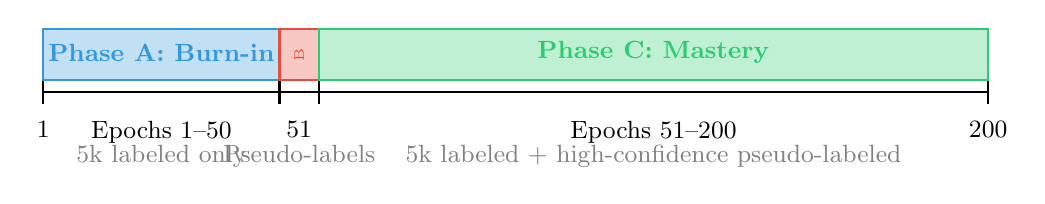
\begin{tikzpicture}[font=\small]
  % Timeline bar
  \draw[thick] (0,0) -- (12,0);
  \foreach \x in {0,3,3.5,12} \draw[thick] (\x, 0.15) -- (\x, -0.15);

  % Phase A
  \fill[burnin!30] (0,0.15) rectangle (3, 0.8);
  \draw[burnin, thick] (0,0.15) rectangle (3, 0.8);
  \node[burnin] at (1.5, 0.5) {\textbf{Phase A: Burn-in}};
  \node[below] at (1.5, -0.25) {Epochs 1--50};
  \node[below, gray] at (1.5, -0.55) {5k labeled only};

  % Phase B
  \fill[highlight!30] (3,0.15) rectangle (3.5, 0.8);
  \draw[highlight, thick] (3,0.15) rectangle (3.5, 0.8);
  \node[highlight, rotate=90, font=\tiny] at (3.25, 0.47) {B};
  \node[below] at (3.25, -0.25) {51};
  \node[below, gray] at (3.25, -0.55) {Pseudo-labels};

  % Phase C
  \fill[mastery!30] (3.5,0.15) rectangle (12, 0.8);
  \draw[mastery, thick] (3.5,0.15) rectangle (12, 0.8);
  \node[mastery] at (7.75, 0.5) {\textbf{Phase C: Mastery}};
  \node[below] at (7.75, -0.25) {Epochs 51--200};
  \node[below, gray] at (7.75, -0.55) {5k labeled + high-confidence pseudo-labeled};

  % Epoch markers
  \node[below] at (0, -0.25) {1};
  \node[below] at (12, -0.25) {200};
\end{tikzpicture}
\end{center}

% ══════════════════════════════════════════════════════════════
\section{The ResNet-50 Architecture}
% ══════════════════════════════════════════════════════════════

\subsection{Residual Block}

The fundamental operation of ResNet-50 is the \emph{bottleneck residual block}. Given input $\mathbf{x}$, the output is:

\begin{equation}
  \mathbf{y} = \mathcal{F}(\mathbf{x}, \{W_i\}) + \mathbf{x}
  \label{eq:residual}
\end{equation}

where $\mathcal{F}$ is the residual function, a composition of three convolutions:

\begin{equation}
  \mathcal{F}(\mathbf{x}) = W_3 * \sigma\!\left( \text{BN}\!\left( W_2 * \sigma\!\left( \text{BN}( W_1 * \mathbf{x} ) \right) \right) \right)
\end{equation}

The channel dimensions for each bottleneck block follow the pattern $C \to C/4 \to C/4 \to C$ for the $1\!\times\!1$, $3\!\times\!3$, and $1\!\times\!1$ convolutions respectively, achieving a \emph{4$\times$ channel reduction} inside the block.

When input/output dimensions differ (e.g., when stride $> 1$), a learned shortcut projection $W_s$ is used:

\begin{equation}
  \mathbf{y} = \mathcal{F}(\mathbf{x}, \{W_i\}) + W_s \mathbf{x}
\end{equation}

\subsection{Full Network Composition}

ResNet-50 applies $L=4$ macro-stages, each containing $[3, 4, 6, 3]$ bottleneck blocks. For an STL-10 image $\mathbf{x}_0 \in \mathbb{R}^{3 \times 96 \times 96}$:

\begin{equation}
  h_0 = \text{MaxPool}\!\left(\sigma(\text{BN}(W_{\text{stem}} * \mathbf{x}_0))\right) \in \mathbb{R}^{64 \times 24 \times 24}
\end{equation}

\begin{align}
  h_1 &= \text{Stage}_1(h_0) \in \mathbb{R}^{256 \times 24 \times 24} \\
  h_2 &= \text{Stage}_2(h_1) \in \mathbb{R}^{512 \times 12 \times 12} \\
  h_3 &= \text{Stage}_3(h_2) \in \mathbb{R}^{1024 \times 6 \times 6} \\
  h_4 &= \text{Stage}_4(h_3) \in \mathbb{R}^{2048 \times 3 \times 3}
\end{align}

The final representation is obtained via global average pooling and the linear head:

\begin{equation}
  \mathbf{z} = W_{\text{fc}}\,\text{GAP}(h_4) \in \mathbb{R}^{10}
  \qquad \text{(10 classes for STL-10)}
\end{equation}

% ══════════════════════════════════════════════════════════════
\section{Phase A: Supervised Burn-in (Epochs 1--50)}
% ══════════════════════════════════════════════════════════════

During the burn-in, the teacher trains on the 5,000 labeled examples $\mathcal{D}_L = \{(\mathbf{x}_i, y_i)\}_{i=1}^{5000}$.

\subsection{Loss Function}

Label-smoothed Cross Entropy with smoothing parameter $\varepsilon = 0.1$ and $K = 10$ classes:

\begin{equation}
  \mathcal{L}_{\text{LS}}(\mathbf{z}, y) = -\sum_{k=1}^{K} \tilde{p}(k|y) \log \hat{p}_k
  \label{eq:label_smooth}
\end{equation}

where the smoothed target distribution is:
\begin{equation}
  \tilde{p}(k|y) = (1-\varepsilon)\,\mathbf{1}[k = y] + \frac{\varepsilon}{K}
\end{equation}

and the predicted distribution is $\hat{p}_k = \text{softmax}(\mathbf{z})_k = \frac{e^{z_k}}{\sum_j e^{z_j}}$.

\subsection{CutMix Augmentation}

With probability 0.5, CutMix is applied. Given two samples $(\mathbf{x}_a, y_a)$ and $(\mathbf{x}_b, y_b)$, a rectangular mask $M$ is sampled and:

\begin{equation}
  \tilde{\mathbf{x}} = M \odot \mathbf{x}_a + (1 - M) \odot \mathbf{x}_b
\end{equation}

The mixing ratio $\lambda$ is adjusted for the actual area of the cut box:
\begin{equation}
  \lambda = 1 - \frac{(x_2 - x_1)(y_2 - y_1)}{W \cdot H}
\end{equation}

The crop box coordinates are sampled from a \textbf{Beta distribution}:
\begin{equation}
  \lambda_0 \sim \text{Beta}(\alpha, \alpha), \quad \alpha = 1.0
  \qquad
  r_W = W\sqrt{1 - \lambda_0},\; r_H = H\sqrt{1 - \lambda_0}
\end{equation}

The mixed loss becomes:
\begin{equation}
  \mathcal{L}_{\text{CutMix}} = \lambda\,\mathcal{L}(\mathbf{z}, y_a) + (1 - \lambda)\,\mathcal{L}(\mathbf{z}, y_b)
\end{equation}

\begin{center}
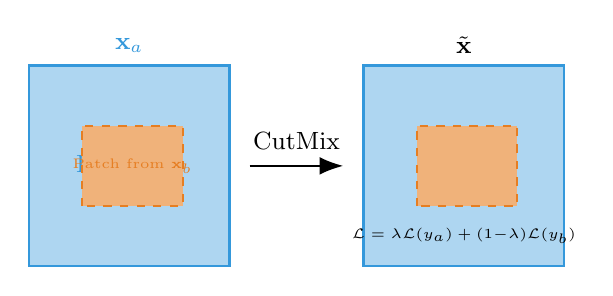
\begin{tikzpicture}[font=\small, scale=0.85]
  % Image A (blue)
  \fill[burnin!40] (0,0) rectangle (3,3);
  \draw[burnin, thick] (0,0) rectangle (3,3);
  \node[burnin] at (1.5,3.3) {$\mathbf{x}_a$};
  \node[burnin] at (1.5,1.5) {Label: $y_a$};

  % Cut region from B
  \fill[gpu2col!60] (0.8,0.9) rectangle (2.3,2.1);
  \draw[gpu2col, thick, dashed] (0.8,0.9) rectangle (2.3,2.1);
  \node[gpu2col, font=\tiny] at (1.55,1.5) {Patch from $\mathbf{x}_b$};

  % Arrow
  \draw[-{Latex[length=3mm]}, thick] (3.3, 1.5) -- (4.7, 1.5);
  \node[above] at (4.0, 1.6) {CutMix};

  % Result
  \fill[burnin!40] (5,0) rectangle (8,3);
  \draw[burnin, thick] (5,0) rectangle (8,3);
  \fill[gpu2col!60] (5.8,0.9) rectangle (7.3,2.1);
  \draw[gpu2col, thick, dashed] (5.8,0.9) rectangle (7.3,2.1);
  \node at (6.5,3.3) {$\tilde{\mathbf{x}}$};
  \node[font=\tiny] at (6.5, 0.45) {$\mathcal{L} = \lambda\mathcal{L}(y_a) + (1{-}\lambda)\mathcal{L}(y_b)$};
\end{tikzpicture}
\end{center}

% ══════════════════════════════════════════════════════════════
\section{Phase B: Pseudo-Label Generation (Epoch 51)}
% ══════════════════════════════════════════════════════════════

At the start of epoch 51, the teacher (frozen) performs inference on the 100,000 unlabeled images $\mathcal{D}_U = \{\mathbf{u}_i\}_{i=1}^{100000}$:

\begin{equation}
  \hat{p}_k^{(i)} = \text{softmax}\!\left(f_\theta(\mathbf{u}_i)\right)_k
\end{equation}

\begin{equation}
  (\hat{c}^{(i)}, \hat{\pi}^{(i)}) = \left(\operatorname*{arg\,max}_k \hat{p}_k^{(i)},\; \max_k \hat{p}_k^{(i)}\right)
\end{equation}

Only images with confidence above threshold $\tau_s$ are retained:

\begin{equation}
  \mathcal{D}_P = \left\{(\mathbf{u}_i, \hat{c}^{(i)}) \;\Big|\; \hat{\pi}^{(i)} > \tau_s \right\}, \quad \tau_s = 0.85
\end{equation}

Because we use a strict threshold, we heavily filter the unlabeled set, retaining only images the model is highly certain about. The expected precision of pseudo-labels under threshold $\tau_s$ is high:

\begin{equation}
  \mathbb{P}[\hat{c}^{(i)} = y_i \mid \hat{\pi}^{(i)} > \tau_s] \gg \frac{1}{K}
\end{equation}

% ══════════════════════════════════════════════════════════════
\section{Phase C: Mastery Training (Epochs 51--200)}
% ══════════════════════════════════════════════════════════════

The combined dataset is:
\begin{equation}
  \mathcal{D}_C = \mathcal{D}_L \cup \mathcal{D}_P
\end{equation}

Training continues from epoch 51 to 200 on $\mathcal{D}_C$ using the identical loss (Eq.~\ref{eq:label_smooth} + CutMix).

\subsection{Optimizer: AdamW}

\begin{equation}
  \theta_{t+1} = \theta_t - \eta_t \frac{\hat{m}_t}{\sqrt{\hat{v}_t} + \epsilon} - \eta_t \lambda_{\text{wd}}\,\theta_t
\end{equation}

where the bias-corrected moment estimates are:
\begin{align}
  \hat{m}_t &= \frac{m_t}{1-\beta_1^t}, \quad m_t = \beta_1 m_{t-1} + (1-\beta_1)g_t \\
  \hat{v}_t &= \frac{v_t}{1-\beta_2^t}, \quad v_t = \beta_2 v_{t-1} + (1-\beta_2)g_t^2
\end{align}

with $\beta_1 = 0.9$, $\beta_2 = 0.999$, $\epsilon = 10^{-8}$, base $\eta_0 = 10^{-3}$, $\lambda_{\text{wd}} = 10^{-4}$.

\subsection{Cosine Annealing LR Schedule}

\begin{equation}
  \eta_t = \eta_{\min} + \frac{1}{2}(\eta_0 - \eta_{\min})\left(1 + \cos\!\frac{\pi t}{T_{\max}}\right)
  \label{eq:cosine}
\end{equation}

with $T_{\max} = 200$, $\eta_{\min} = 0$.

\begin{center}
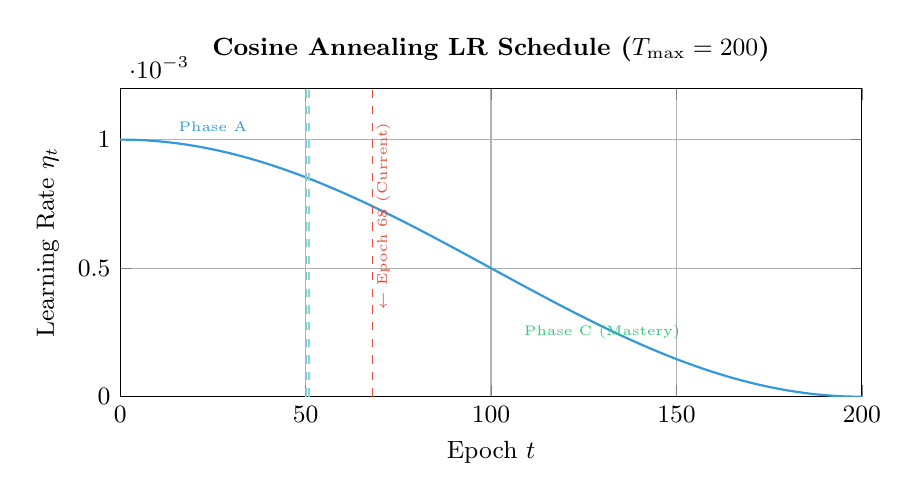
\begin{tikzpicture}
\begin{axis}[
    width=11cm, height=5.5cm,
    xlabel={Epoch $t$},
    ylabel={Learning Rate $\eta_t$},
    title={Cosine Annealing LR Schedule ($T_{\max}=200$)},
    samples=200,
    domain=0:200,
    ymin=0, ymax=0.0012,
    xmin=0, xmax=200,
    xtick={0,50,100,150,200},
    grid=both,
    grid style={line width=0.2pt, draw=gray!30},
    major grid style={line width=0.4pt, draw=gray!60},
    tick label style={font=\small},
    label style={font=\small},
    title style={font=\small\bfseries},
]
  % Cosine curve
  \addplot[burnin, thick] {0.001 * 0.5 * (1 + cos(deg(pi * x / 200)))};

  % Phase A marker
  \addplot[burnin!60, dashed, thick] coordinates {(50, 0) (50, 0.0012)};
  \node[burnin, font=\tiny] at (axis cs:25, 0.00105) {Phase A};

  % Phase C marker
  \addplot[mastery!60, dashed, thick] coordinates {(51, 0) (51, 0.0012)};
  \node[mastery, font=\tiny] at (axis cs:130, 0.00025) {Phase C (Mastery)};

  % Epoch 68 (current position) marker
  \addplot[highlight, dashed] coordinates {(68, 0) (68, 0.0012)};
  \node[highlight, font=\tiny, rotate=90] at (axis cs:71, 0.0007) {$\leftarrow$ Epoch 68 (Current)};
\end{axis}
\end{tikzpicture}
\end{center}

\subsection{Gradient Clipping}

To prevent gradient explosions when training on noisy pseudo-labels, gradient norms are clipped:

\begin{equation}
  g_t \leftarrow g_t \cdot \min\!\left(1,\; \frac{G_{\max}}{\|g_t\|_2}\right), \quad G_{\max} = 1.0
\end{equation}

% ══════════════════════════════════════════════════════════════
\section{Multi-GPU Data Parallelism}
% ══════════════════════════════════════════════════════════════

\subsection{Mathematical Formulation}

With $P = 2$ GPUs (T4 $\times$ 2), a mini-batch $\mathcal{B}$ of size $B = 128$ is partitioned:

\begin{equation}
  \mathcal{B} = \mathcal{B}_1 \cup \mathcal{B}_2, \quad |\mathcal{B}_p| = B/P = 64
\end{equation}

Each GPU $p$ holds a \emph{replica} of the model $f_{\theta^{(p)}}$ and computes its own loss:

\begin{equation}
  \mathcal{L}_p = \frac{1}{|\mathcal{B}_p|}\sum_{(\mathbf{x},y)\in\mathcal{B}_p} \ell(f_{\theta^{(p)}}(\mathbf{x}), y)
\end{equation}

Gradients are computed independently on each device:
\begin{equation}
  g_p = \nabla_{\theta^{(p)}} \mathcal{L}_p
\end{equation}

After the backward pass, \textbf{gradients are averaged and aggregated (AllReduce)} on GPU~0:

\begin{equation}
  \bar{g} = \frac{1}{P}\sum_{p=1}^{P} g_p
\end{equation}

The optimizer step runs once on GPU~0 using $\bar{g}$ and updated weights $\theta^*$ are \textbf{broadcast} back to all replicas before the next iteration:

\begin{equation}
  \theta^{(p)} \leftarrow \theta^* = \text{AdamW}(\theta_0,\, \bar{g}), \quad \forall p
\end{equation}

This is mathematically equivalent to training on the full batch $\mathcal{B}$ on a single GPU, but each forward/backward pass takes roughly $\frac{1}{P}$ of the time.

\subsection{Implementation Note: State Dict Keys}

\texttt{nn.DataParallel} normally prepends \texttt{module.} to every key in the state dict. To preserve checkpoint portability, the training script explicitly strips this prefix before saving:

\begin{equation}
  \texttt{save\_state} = \theta^*.state\_dict()
  \quad\text{(via \texttt{model.module.state\_dict()} when wrapped)}
\end{equation}

\begin{center}
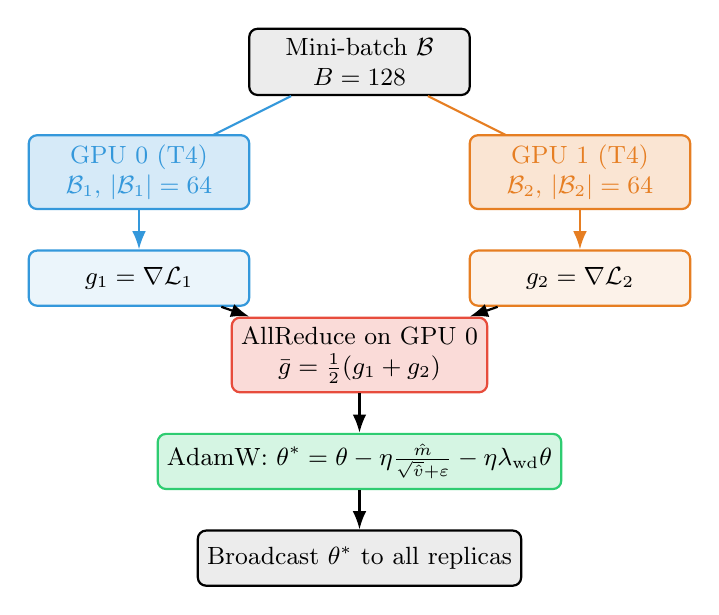
\begin{tikzpicture}[
  font=\small,
  box/.style={rectangle, rounded corners=3pt, thick, draw, minimum width=2.8cm, minimum height=0.7cm, align=center},
]

  % Data source
  \node[box, fill=gray!15] (data) at (0,0) {Mini-batch $\mathcal{B}$\\ $B = 128$};

  % Scatter arrows
  \draw[-{Latex}, thick, burnin] (data) -- ++(-2.8, -1.4) node[box, fill=burnin!20, draw=burnin] (gpu1) {GPU 0 (T4)\\ $\mathcal{B}_1$, $|\mathcal{B}_1|=64$};
  \draw[-{Latex}, thick, gpu2col] (data) -- ++(2.8, -1.4) node[box, fill=gpu2col!20, draw=gpu2col] (gpu2) {GPU 1 (T4)\\ $\mathcal{B}_2$, $|\mathcal{B}_2|=64$};

  % Forward/backward
  \node[box, fill=burnin!10, draw=burnin, below=0.5cm of gpu1] (grad1) {$g_1 = \nabla\mathcal{L}_1$};
  \node[box, fill=gpu2col!10, draw=gpu2col, below=0.5cm of gpu2] (grad2) {$g_2 = \nabla\mathcal{L}_2$};

  \draw[-{Latex}, thick, burnin] (gpu1) -- (grad1);
  \draw[-{Latex}, thick, gpu2col] (gpu2) -- (grad2);

  % AllReduce
  \node[box, fill=highlight!20, draw=highlight, below=2.8cm of data] (reduce) {AllReduce on GPU 0\\ $\bar{g} = \frac{1}{2}(g_1 + g_2)$};

  \draw[-{Latex}, thick] (grad1) -- (reduce);
  \draw[-{Latex}, thick] (grad2) -- (reduce);

  % Optimizer step
  \node[box, fill=mastery!20, draw=mastery, below=0.5cm of reduce] (optim) {AdamW: $\theta^* = \theta - \eta\frac{\hat{m}}{\sqrt{\hat{v}}+\varepsilon} - \eta\lambda_\text{wd}\theta$};

  \draw[-{Latex}, thick] (reduce) -- (optim);

  % Broadcast back
  \node[box, fill=gray!15, below=0.5cm of optim] (bcast) {Broadcast $\theta^*$ to all replicas};
  \draw[-{Latex}, thick] (optim) -- (bcast);

\end{tikzpicture}
\end{center}

% ══════════════════════════════════════════════════════════════
\section{Expected Validation Accuracy Trajectory}
% ══════════════════════════════════════════════════════════════

The following figure illustrates the expected qualitative accuracy curve from the combination of pseudo-labeling and cosine annealing, along with the current checkpoint state.

\begin{center}
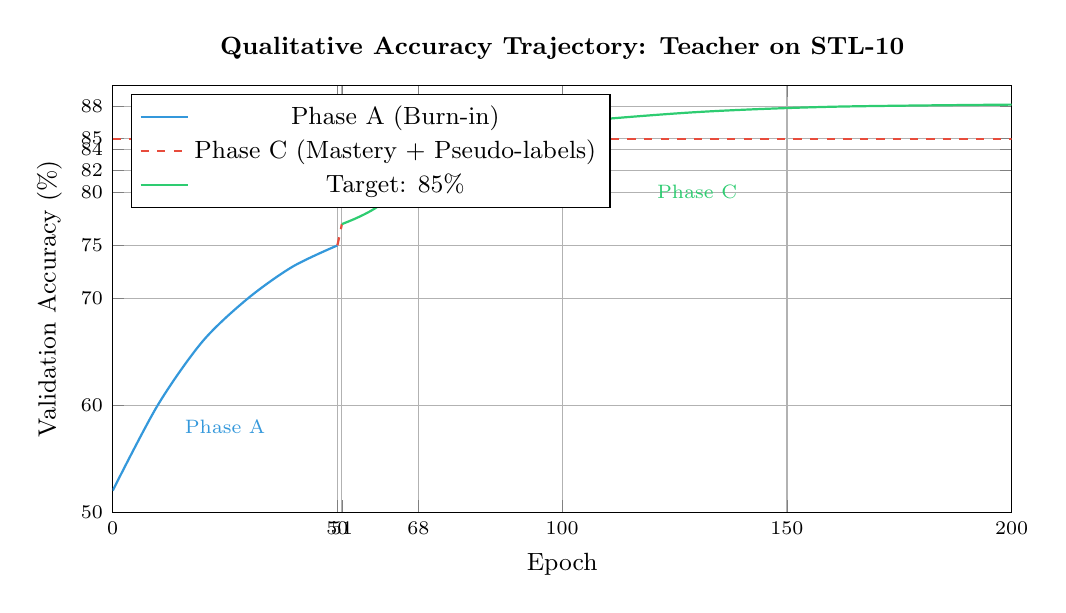
\begin{tikzpicture}
\begin{axis}[
    width=13cm, height=7cm,
    xlabel={Epoch}, ylabel={Validation Accuracy (\%)},
    title={Qualitative Accuracy Trajectory: Teacher on STL-10},
    xmin=0, xmax=200,
    ymin=50, ymax=90,
    xtick={0,50,51,68,100,150,200},
    xticklabels={0,50,51,68,100,150,200},
    ytick={50,60,70,75,80,82,84,85,88},
    grid=both,
    grid style={line width=0.2pt, draw=gray!30},
    major grid style={line width=0.4pt, draw=gray!60},
    tick label style={font=\scriptsize},
    label style={font=\small},
    title style={font=\small\bfseries},
    legend style={font=\small, at={(0.02,0.98)}, anchor=north west},
]
  % Phase A: slow climb 1-50
  \addplot[burnin, thick, smooth] coordinates {
    (0, 52)(10, 60)(20,66)(30,70)(40,73)(50,75)
  };
  \addlegendentry{Phase A (Burn-in)};

  % Phase B transition jump at 51
  \addplot[highlight, thick, dashed] coordinates {(50,75)(51,77)};

  % Phase C: 51-200
  \addplot[mastery, thick, smooth] coordinates {
    (51,77)(60,79)(68,84)(80,85.5)(100,86.5)(130,87.5)(160,88)(200,88.2)
  };
  \addlegendentry{Phase C (Mastery + Pseudo-labels)};

  % 85% target line
  \addplot[highlight, dashed, thick, domain=0:200] {85};
  \addlegendentry{Target: 85\%};

  % Current epoch marker
  \addplot[only marks, mark=*, mark size=3pt, highlight] coordinates {(68, 84)};
  \node[highlight, font=\scriptsize] at (axis cs:80, 83.2) {Current (Ep. 68, 84\%)};

  % Phase labels
  \node[burnin, font=\scriptsize] at (axis cs:25, 58) {Phase A};
  \node[mastery, font=\scriptsize] at (axis cs:130, 80) {Phase C};

\end{axis}
\end{tikzpicture}
\end{center}

\begin{table}[h]
\centering
\caption{Summary of training hyperparameters for the Ultimate Teacher Model.}
\begin{tabular}{@{}lll@{}}
\toprule
\textbf{Hyperparameter} & \textbf{Symbol} & \textbf{Value} \\
\midrule
Base learning rate & $\eta_0$ & $1 \times 10^{-3}$ \\
Weight decay & $\lambda_{\text{wd}}$ & $1 \times 10^{-4}$ \\
Adam $\beta_1$ & $\beta_1$ & 0.9 \\
Adam $\beta_2$ & $\beta_2$ & 0.999 \\
LR schedule & — & Cosine Annealing \\
$T_{\max}$ & $T_{\max}$ & 200 \\
Label smoothing & $\varepsilon$ & 0.1 \\
CutMix probability & — & 0.5 \\
CutMix $\alpha$ & $\alpha$ & 1.0 \\
Pseudo-label threshold & $\tau_s$ & 0.85 \\
Max gradient norm & $G_{\max}$ & 1.0 \\
Batch size (total) & $B$ & 128 \\
Batch size per GPU & $B/P$ & 64 \\
\# GPUs & $P$ & 2 (T4 $\times$ 2) \\
\bottomrule
\end{tabular}
\end{table}

% ══════════════════════════════════════════════════════════════
\section{Full Training Algorithm}
% ══════════════════════════════════════════════════════════════

\begin{algorithm}[H]
\caption{Ultimate Teacher Training Pipeline}
\begin{algorithmic}[1]
\State Initialize $\theta \sim \mathcal{N}(0, \sigma^2)$ (or warm-restart weights)
\State Load checkpoint if available; set $t \leftarrow t_{\text{resume}}$
\State Initialize replicas $\theta^{(p)} \leftarrow \theta$ on each GPU $p$
\For{$t = 1$ to $N = 200$}
  \If{$t = N_{\text{burn-in}} + 1$ \textbf{and} $\mathcal{D}_P = \emptyset$}
    \State \textbf{Phase B:} Run inference on $\mathcal{D}_U$; collect $\mathcal{D}_P = \{(\mathbf{u}, \hat{c}) : \hat{\pi} > \tau_s\}$
  \EndIf
  \State $\mathcal{D}_{\text{active}} \leftarrow \mathcal{D}_L$ if $t \leq N_{\text{burn-in}}$ else $\mathcal{D}_L \cup \mathcal{D}_P$
  \For{each mini-batch $\mathcal{B} \sim \mathcal{D}_{\text{active}}$}
    \State Scatter $\mathcal{B}$ to GPUs: $\mathcal{B}_p = \mathcal{B}[(p-1)B/P : pB/P]$
    \For{each GPU $p$ \textbf{in parallel}}
      \If{\texttt{rand()} $> 0.5$} apply CutMix to $\mathcal{B}_p$
      \EndIf
      \State $\mathcal{L}_p \leftarrow$ label-smoothed CE (+ CutMix mixture) on $\mathcal{B}_p$
      \State $g_p \leftarrow \nabla_\theta \mathcal{L}_p$
    \EndFor
    \State $\bar{g} \leftarrow \frac{1}{P}\sum_p g_p$ \hfill (AllReduce)
    \State Clip: $\bar{g} \leftarrow \bar{g} \cdot \min(1, G_{\max}/\|\bar{g}\|_2)$
    \State $\theta \leftarrow \text{AdamW}(\theta, \bar{g})$; broadcast $\theta$ to all $\theta^{(p)}$
  \EndFor
  \State $\eta_t \leftarrow \frac{\eta_0}{2}\!\left(1 + \cos\!\frac{\pi t}{T_{\max}}\right)$ \hfill (Cosine Annealing)
  \State Evaluate on validation set; save best and latest checkpoint
\EndFor
\State \Return $\theta^*$ (best validation accuracy weights)
\end{algorithmic}
\end{algorithm}

\end{document}
